\documentclass[12pt,a4paper, openany]{book}
\makeatletter
\setlength{\unitlength}{1cm}
\usepackage[english]{babel}

\usepackage[latin1]{inputenc}
\usepackage{epsfig}
\usepackage{bezier}
\usepackage{xr}
\usepackage{srcltx}
\usepackage{float}
\usepackage{rotating}
\usepackage{array}


\usepackage{amsmath}
\usepackage{amsthm}
\usepackage{amssymb}
\usepackage{amsfonts}

\usepackage{booktabs}  % for table in Latex
\usepackage{theorem}
\usepackage{longtable}
\usepackage{ssm}
\usepackage{pifont}
\usepackage{verbatim}
\usepackage{latexsym}
\usepackage{ifthen}%\externaldocument[LSG-]{loesung}
\usepackage{enumerate}
\usepackage{enumitem} % Customize enumerate, itemize and description environments
\setlist[enumerate]{topsep=2pt, itemsep=5pt}
\setlist[itemize]{topsep=0pt, itemsep=2pt, midpenalty=10000}

\usepackage{psfrag}   % for the letters in .eps figures 

\usepackage{graphics} % for pdf, bitmapped graphics files
\usepackage{graphicx}
\usepackage{lscape}
\usepackage{tikz}
\usepackage{color}
\definecolor{hell_blau}{RGB}{0, 102, 255}

\usepackage{framed}

\usepackage[e]{esvect} % Darstellung von Vektoren

\usepackage{tabularx}	% Tabellen mit Größenangaben
\newcolumntype{C}[1]{>{\centering\arraybackslash}p{#1}}
\newcolumntype{L}[1]{>{\arraybackslash}p{#1}}

\usepackage{multirow}	% Zellen einer Tabelle in mehrere Zeilen unterteilen

\usepackage{rotating} % Bilder quer auf Seite darstellen
\usepackage{lscape}		% 
\usepackage{fancyhdr}
\setlength{\headheight}{30pt}

\usepackage{setspace}

\usepackage{cancel} % Zum Streichen von Termen in Gleichungen
\renewcommand{\CancelColor}{\color{red}} %change cancel color to red

\usepackage{caption}
\captionsetup{
  justification=centering,
  singlelinecheck=off
}
\usepackage[labelformat=simple]{subcaption}
\renewcommand\thesubfigure{(\alph{subfigure})}


% Zur Formatierung von Titeln usw.:
\usepackage{titlesec}
\titleformat{\chapter}[frame]{\normalfont\LARGE\bfseries}
    {}{5pt}{\centering \sc}
		\titlespacing{\chapter}{0cm}{-2cm}{0cm}

%\usepackage[babel,german=quotes]{csquotes}
\usepackage[
bibstyle=numeric-comp,    % Zitierstil
isbn=false,                % ISBN nicht anzeigen, gleiches geht mit nahezu allen anderen Feldern
%pagetracker=true,          % ebd. bei wiederholten Angaben (false=ausgeschaltet, page=Seite, spread=Doppelseite, true=automatisch)
maxbibnames=50,            % maximale Namen, die im Literaturverzeichnis angezeigt werden (ich wollte alle)
maxcitenames=3,            % maximale Namen, die im Text angezeigt werden, ab 4 wird u.a. nach den ersten Autor angezeigt
autocite=inline,           % regelt Aussehen für \autocite (inline=\parancite)
block=space,               % kleiner horizontaler Platz zwischen den Feldern
backref=true,              % Seiten anzeigen, auf denen die Referenz vorkommt
backrefstyle=three+,       % fasst Seiten zusammen, z.B. S. 2f, 6ff, 7-10
date=short,                % Datumsformat
giveninits=true,
backend=biber]{biblatex}
\addbibresource{Literatur.bib}
\setlength{\bibitemsep}{10pt}
%Autorenformat ändern
%\DeclareNameFormat{default}{%Vollzitate
%  \ifnum\value{listcount}=1\relax
%    \iffirstinits
%      {\usebibmacro{name:last-first}{#1}{#4}{#5}{#7}}
%      {\usebibmacro{name:last-first}{#1}{#3}{#5}{#7}}%
%  \else
%    \iffirstinits
%      {\usebibmacro{name:first-last}{#1}{#4}{#5}{#7}}
%      {\usebibmacro{name:first-last}{#1}{#3}{#5}{#7}}%
%  \fi
%  \usebibmacro{name:andothers}} 
	

\usepackage[babel,german=quotes]{csquotes}
\AtBeginBibliography{%
  \renewcommand*{\mkbibnamelast}[1]{\textsc{#1}}}
	
\usepackage[colorlinks=true, linkcolor=blue, urlcolor=hell_blau, citecolor=red]{hyperref}


%\renewcommand{\textfraction}{0.0}
%\renewcommand{\topfraction}{1.0}
%\renewcommand{\bottomfraction}{1.0}
%\renewcommand{\thefootnote}{\arabic{footnote})~}
%\renewcommand{\labelenumi}{(\arabic{enumi})}
%%%%%%%%%%%%%%%%%%%%%%%%%%%%%%%%%%%%%%%%%%%%%%%%%%%%%%%%%%%%%%%%%%%%%%%%%%%%%
% 	Section for Page Layout
%%%%%%%%%%%%%%%%%%%%%%%%%%%%%%%%%%%%%%%%%%%%%%%%%%%%%%%%%%%%%%%%%%%%%%%%%%%%%
\singlespacing
%\onehalfspacing
%\doublespacing

\pagestyle{plain}

%%%%%%%%%%%%%%%%%%%%%
% 	all about the text and page style
%		see Latex_layout.svg
%   1. one inch + \hoffset
%   2. one inch + \voffset
%   3. \oddsidemargin = 31pt
%   4. \topmargin = 20pt
%   5. \headheight = 12pt
%   6. \headsep = 25pt
%   7. \textheight = 592pt
%   8. \textwidth = 390pt
%   9. \marginparsep = 10pt
%  10. \marginparwidth = 35pt
%  11. \footskip = 30pt

%		DIN A4 : height x width: 29.7 cm x 21.0 cm
%		1 inch = 2.54 cm
%		define page layout using package "`setlength"'
\setlength{\hoffset}{-0.54cm}  
\setlength{\voffset}{-0.54cm}  
\setlength{\oddsidemargin}{+0.3cm}
\setlength{\evensidemargin}{-0.3cm} 
\setlength{\topmargin}{0.0cm}
\setlength{\headheight}{0.6cm}
\setlength{\headsep}{1cm}
\setlength{\textheight}{23.6cm}
\setlength{\textwidth}{17.0cm}
\setlength{\marginparsep}{0.0cm}  
\setlength{\marginparwidth}{0cm}  
\setlength{\footskip}{1cm}

% additional outlay definitions
%	no indent for new paragraph by \\
\setlength{\parindent}{0mm}
\setlength{\marginparpush}{0cm}  

%%%%%%%%%%%%%%%%%%%%%%%%%%%%%%%%%%%%%%%%%%%%%%%%%%%%%%%%%%%%%%



%%%%%%%%%%%%%%%%%%%%%%%%%%%%%%%%%%%%%%%%%%%%%%%%%%%%%%%%%%%%%%%%%%%%%%%%%%%%%
%    	Set line spacing  (by Multiplier ... 1.5 here)
%%%%%%%%%%%%%%%%%%%%%%%%%%%%%%%%%%%%%%%%%%%%%%%%%%%%%%%%%%%%%%%%%%%%%%%%%%%%%
%\renewcommand{\baselinestretch}{1.05}
%%%%%%%%%%%%%%%%%%%%%%%%%%%%%%%%%%%%%%%%%%%%%%%%%%%%%%%%%%%%%%%%%%%%%%%%%%%%%

%%%%%%%%%%%%%%%%%%%%%%%%%%%%%%%%%%%%%%%%%%%%%%%%%%%%%%%%%%%%%%%%%%%%%%%%%%%%%
%    	Fancy Page Layout with Fancy Header
%%%%%%%%%%%%%%%%%%%%%%%%%%%%%%%%%%%%%%%%%%%%%%%%%%%%%%%%%%%%%%%%%%%%%%%%%%%%%
\pagestyle{fancy}

\let\origdoublepage\cleardoublepage
\newcommand{\clearemptydoublepage}{%
  \clearpage
  {\pagestyle{empty}\origdoublepage}%
}
%%%%%%%%%%%%%%%%%%%%%%%%%%%%%%%%%%%%%%%%%%%%%%%%%%%%%%%%%%%%%%%%%%%%%%%%%%%%%

%%%%%%%%%%%%%%%%%%%%%%%%%%%%%%%%%%%%%%%%%%%%%%%%%%%%%%%%%%%%%%%%%%%%%%%%%%%%%
% 	all about head & foot rule 
\renewcommand{\headrulewidth}{0.5pt}
\renewcommand{\footrulewidth}{0.5pt}
\setlength{\headwidth}{\textwidth}

%\renewcommand{\rightmark}{\thesection\ #1}
%\renewcommand{\leftmark}{Chapter \thechapter}
%\renewcommand{\chaptermark}[1]{\markboth{Chapter~\thechapter:\ #1}{}}
\renewcommand{\sectionmark}[1]{\markboth{\textsc{\thesection.~#1}}{}}
\renewcommand{\subsectionmark}[1]{\markright{\textsc{\thesubsection.~#1}}}
%\renewcommand{\sectionmark}[1]{\markright{\thesection.~#1}{}}
%%%%%%%%%%%%%%%%%%%%%%%%%%%%%%%%%%%%%%%%%%%%%%%%%%%%%%%%%%%%%%%%%%%%%%%%%%%%%

%%%%%%%%%%%%%%%%%%%%%%%%%%%%%%%%%%%%%%%%%%%%%%%%%%%%%%%%%%%%%%%%%%%%%%%%%%%%%
% 	all about shown content in header
%\lhead[\bfseries Page \thepage]{\bfseries\rightmark}
\lhead[\fancyplain{}{\leftmark}]{\fancyplain{}{}}
%\rhead[\bfseries\leftmark]{\bfseries Page \thepage}
\rhead[\fancyplain{}{}]{\fancyplain{}{\rightmark}}
\cfoot{--~\thepage~--}
% \rfoot{\bfseries\thepage}
%%%%%%%%%%%%%%%%%%%%%%%%%%%%%%%%%%%%%%%%%%%%%%%%%%%%%%%%%%%%%%%%%%%%%%%%%%%%%

\fancypagestyle{plain}{%
\fancyhf{} % clear all header and footer fields
\cfoot{--~\thepage~--} % except the center
\renewcommand{\headrulewidth}{0pt}
\renewcommand{\footrulewidth}{0.5pt}}


%%%%%%%%%%%%%%%%%%%%%%%%%%%%%%% AMSTHM new commands %%%%%%%%%%%%%%%%%%%%%%%%%%
%\newtheoremstyle{MyPlain}% name
%  {9pt}%      Space above, empty = `usual value'
% 	{9pt}%      Space below
%  {\itshape}% Body font
%  {\parindent}%         Indent amount (empty = no indent, \parindent = para indent)
%  {\bfseries}% Thm head font
%  {}%        Punctuation after thm head
%  {0.5em}% Space after thm head: \newline = linebreak
%  {}%         Thm head spec 
%
%\theoremstyle{MyPlain} %default[chapter]

%\newtheorem{theorem}{Theorem}[Section]
%\newtheorem{proposition}[theorem]{Proposition}
%\newtheorem{lemma}[theorem]{Lemma}
%\newtheorem{corollary}[theorem]{Corollary}
%\newtheorem{definition}[theorem]{Definition}
%%\newtheorem*{definition*}{Definition}
%\newtheorem{remark}[theorem]{Remark}
%\newtheorem{claim}[theorem]{Claim}
%\newtheorem{example}[theorem]{Example}
%\newtheorem{examples}[theorem]{Examples}
%\newtheorem{assumption}[theorem]{Assumption}
%\newtheorem{motivation}[theorem]{Motivation}
%\newtheorem{property}{Property}
%\newtheorem{note}[theorem]{Note}
 %
%%%%%%%%%%%%%%%%%%%%%%%%%%%%%%% AMSTHM new commands %%%%%%%%%%%%%%%%%%%%%%%%%%
%
%
%%%%%%%%%%%%%%%%%%%%%%%%%%%%%%%%%%%%%%%%%%%%%%%%%%%%%%%%%%%%%%%%%%%%%%%%%%%%%
%	(RE-)DEFINE NEW MATH EXPRESSIONS

%	Define new math operators
%\DeclareMathOperator{\kern}{kern} %somewhere already defined
\DeclareMathOperator{\essinf}{ess-inf}
\DeclareMathOperator*{\esssup}{ess-sup}
\DeclareMathOperator*{\supr}{sup}
\DeclareMathOperator{\dist}{dist}
\DeclareMathOperator{\diag}{diag}
\DeclareMathOperator{\graph}{graph}
\DeclareMathOperator{\sign}{sign}
\DeclareMathOperator{\rank}{rank}
\DeclareMathOperator{\sat}{sat}
\DeclareMathOperator{\spec}{spec}
\DeclareMathOperator{\loc}{loc}
\DeclareMathOperator{\grad}{grad}
\DeclareMathOperator{\fin}{fin}
\DeclareMathOperator{\vol}{vol}
\DeclareMathOperator{\col}{col}
\DeclareMathOperator{\row}{row}
\DeclareMathOperator{\lin}{lin}

%	Abbreviate sets, compact sets  (of numbers, ...)
\newcommand{\N}{\mathbb{N}}
\newcommand{\B}{\mathbb{B}}
\newcommand{\Z}{\mathbb{Z}}
\newcommand{\Q}{\mathbb{Q}}
\newcommand{\R}{\mathbb{R}}
\newcommand{\Rp}{\mathbb{R}_{\geq 0}}
\newcommand{\Rsp}{\mathbb{R}_{> 0}}
\newcommand{\C}{\mathbb{C}}
\newcommand{\Cn}{\mathbb{C}_{< 0}}
\newcommand{\Czp}{\mathbb{C}_{\geq 0}}
%	compact set
\newcommand{\cset}[1]{\mathfrak{#1}}
%	open set
\newcommand{\oset}[1]{\mathcal{#1}}
%	function set
\newcommand{\fset}[1]{\mathcal{#1}}
%	system class 
\newcommand{\sclass}[1]{\mathcal{#1}}
%	operator class 
\newcommand{\oclass}[1]{\mathcal{#1}}
%	boundary set
\newcommand{\bset}[1]{\mathcal{#1}}

%	often used symbols or nomenclature

%	special for Praktikum ET S2
\newcommand{\eff}{\rm{eff}}
\newcommand{\str}{\rm{STR}}


\newcommand{\myref}{\rm{ref}}
%	my (gain) scaling
\newcommand{\gsc}{\varsigma}
\newcommand{\gscmin}{\underline{\varsigma}}
%	high-frequency gain
\newcommand{\hfg}{\gamma_0}
%	steady-state gain
\newcommand{\ssg}{\gamma_{\infty}}
%	root locus center
\newcommand{\rlc}{\Xi}
%	boundaries
%\newcommand{\pF}{\mathcal{F}}
\newcommand{\pF}{\psi}

\newcommand{\pFE}{\psi_E}
\newcommand{\pFphi}{\mathcal{F}_{\phi}}
\newcommand{\dx}[1]{{\rm \, d} #1 \,}
\newcommand{\fdiff}[2]{\frac{\textrm{d}^{#1}}{\textrm{d}#2^{#1}}\,}
\newcommand{\fpartial}[2]{\frac{\partial^{#1}}{\partial #2^{#1}}\,}
\newcommand{\fpartials}[3]{\frac{\partial^{#1}{#3}}{\partial #2^{#1}}\,}
\newcommand{\eps}{\varepsilon}
\newcommand{\foraa}{\textrm{for~a.a.~}}
%	certain instants of time
\newcommand{\tstar}{t^{\star}}
\newcommand{\tlstar}{t_{\star}}
%	motion control objectives
\newcommand{\trise}[1]{t_{y(\cdot),{#1}}^{r}}
\newcommand{\triseref}[1]{t_{{\myref},{#1}}^{r}}
\newcommand{\tset}[1]{t_{y(\cdot),{#1}}^{s}}
\newcommand{\tsetref}[1]{t_{{\myref},{#1}}^{s}}
\newcommand{\os}{\Delta_{y(\cdot)}^{os}}
\newcommand{\osref}{\Delta_{\myref}^{os}}
%	gains 
\newcommand{\kmax}{k_{\max}}
\newcommand{\kinf}{k_{\infty}}
\newcommand{\kmin}{k_{\min}}
\newcommand{\kstar}{k^{\star}}
% control
\newcommand{\ufeas}{u_{\rm{feas}}}
\newcommand{\uhat}{\hat{u}}

\newcommand{\setdef}[2]{\left\{\ #1\ \left|\vphantom{#1}\ #2\ \right.\right\}}

%	function spaces
\newcommand{\Lp}[1]{\fset{L}^{#1}}
\newcommand{\Lone}{\fset{L}^{1}}
\newcommand{\Loneloc}{\fset{L}^{1}_{\loc}}
\newcommand{\Ltwo}{\fset{L}^{2}}
\newcommand{\Linf}{\fset{L}^{\infty}}
\newcommand{\Linfloc}{\fset{L}^{\infty}_{\loc}}
\newcommand{\Ck}{\fset{C}^{k}}
\newcommand{\Czero}{\fset{C}}
\newcommand{\Cone}{\fset{C}^{1}}
\newcommand{\Cinf}{\fset{C}^{\infty}}
\newcommand{\Wkinf}{\fset{W}^{k,\infty}}
\newcommand{\Woneinf}{\fset{W}^{1,\infty}}
\newcommand{\Wtwoinf}{\fset{W}^{2,\infty}}


%	lapace
\newcommand{\laplaceT}[1]{\mathscr{L}\left\{#1\right\}}

%	myVector = \mv
\newcommand{\mv}[1]{\boldsymbol{#1}}
%	myMatrix = \mm
\newcommand{\mm}[1]{\boldsymbol{#1}}
%	myOperator = \mO
\newcommand{\mo}[1]{\boldsymbol{\mathfrak{#1}}}
%	norm ||.||
\newcommand{\norm}[1]{\left\lVert #1 \right\rVert}
% ||.||_infty
\newcommand{\esnorm}[1]{\lVert #1 \rVert_{\infty}}
\newcommand{\Lnorm}[2]{\lVert #2 \rVert_{\fset{L}^{#1}}}
%	inner product <.,.>
\newcommand{\iproduct}[2]{\langle #1,\, #2 \rangle}
%	for dimensions e.g. [Nm]
\newcommand{\di}[1]{\left[\rm{#1}\right]}

% for typewriting:
\newcommand{\tw}[1]{{\tt #1}}

%	system classes
\newcommand{\Sonelin}{\sclass{S}_1^{\lin}}
\newcommand{\Stwolin}{\sclass{S}_2^{\lin}}
\newcommand{\Sone}{\sclass{S}_1}
\newcommand{\Stwo}{\sclass{S}_2}

%	Dimensions
\newcommand{\Ohm}{\Omega}
%
%	CHANGE ENUMERATE NUMBERING
\renewcommand{\labelenumi}{\arabic{enumi}.)}
%\renewcommand{\labelenumii}{(\alph{enumii})}
% 	

% define colors for TIKZ
\definecolor{brown}{RGB}{153, 51,0} %	from Matlab (0.6*255, 0.2*255,0)
\definecolor{orange}{RGB}{255, 127.5,0}
\definecolor{gray}{RGB}{127.5, 127.5,127.5}
%\definecolor{r2}{RGB}{252,177,49}
%\definecolor{r3}{RGB}{35,34,35}
%\definecolor{r4}{RGB}{0,157,87}
%\definecolor{r5}{RGB}{238,50,78}


%	define macros to draw colored lines with TIKZ package
\newcommand{\blueline}{\protect\tikz{\protect\draw[very thick,blue] (0,-0.5ex)(0,0)--(4ex,0);}}
\newcommand{\orangeline}{\protect\tikz{\protect\draw[very thick,orange] (0,-0.5ex)(0,0)--(4ex,0);}}
\newcommand{\brownline}{\protect\tikz{\protect\draw[very thick,brown] (0,-0.5ex)(0,0)--(4ex,0);}}
\newcommand{\bluedashdottedline}{\protect\tikz{\protect\draw[very thick,blue,dashdotted] (0,-0.5ex)(0,0)--(4ex,0);}}
\newcommand{\bluedottedline}{\protect\tikz{\protect\draw[very thick,blue,dotted] (0,-0.5ex)(0,0)--(4ex,0);}}
\newcommand{\bluedashedline}{\protect\tikz{\protect\draw[very thick,dashed,blue] (0,-0.5ex)(0,0)--(4ex,0);}}
\newcommand{\cyanline}{\protect\tikz{\protect\draw[very thick,cyan] (0,-0.5ex)(0,0)--(4ex,0);}}
\newcommand{\cyandashdottedline}{\protect\tikz{\protect\draw[very thick,dashdotted,cyan] (0,-0.5ex)(0,0)--(4ex,0);}}
\newcommand{\cyandashedline}{\protect\tikz{\protect\draw[very thick,dashed,cyan] (0,-0.5ex)(0,0)--(4ex,0);}}
\newcommand{\cyandottedline}{\protect\tikz{\protect\draw[very thick,dotted,cyan] (0,-0.5ex)(0,0)--(4ex,0);}}
\newcommand{\magentaline}{\protect\tikz{\protect\draw[very thick,magenta] (0,-0.5ex)(0,0)--(4ex,0);}}
\newcommand{\magentadashedline}{\protect\tikz{\protect\draw[very thick, dashed,magenta] (0,-0.5ex)(0,0)--(4ex,0);}}
\newcommand{\magentdaottedline}{\protect\tikz{\protect\draw[very thick, dotted,magenta] (0,-0.5ex)(0,0)--(4ex,0);}}
\newcommand{\magentadashdottedline}{\protect\tikz{\protect\draw[very thick, dashdotted,magenta] (0,-0.5ex)(0,0)--(4ex,0);}}
\newcommand{\greenline}{\protect\tikz{\protect\draw[very thick,green] (0,-0.5ex)(0,0)--(4ex,0);}}
\newcommand{\blackline}{\protect\tikz{\protect\draw[very thick,black] (0,-0.5ex)(0,0)--(4ex,0);}}
\newcommand{\blackdashedline}{\protect\tikz{\protect\draw[very thick,dashed,black] (0,-0.5ex)(0,0)--(4ex,0);}}
\newcommand{\blackdottedline}{\protect\tikz{\protect\draw[very thick,dotted,black] (0,-0.5ex)(0,0)--(4ex,0);}}
\newcommand{\blackdashdottedline}{\protect\tikz{\protect\draw[very thick,black,dashdotted] (0,-0.5ex)(0,0)--(4ex,0);}}
\newcommand{\redline}{\protect\tikz{\protect\draw[very thick,red] (0,-0.5ex)(0,0)--(4ex,0);}}
\newcommand{\reddottedline}{\protect\tikz{\protect\draw[very thick,dotted,red] (0,-0.5ex)(0,0)--(4ex,0);}}
\newcommand{\reddashedline}{\protect\tikz{\protect\draw[very thick,dashed,red] (0,-0.5ex)(0,0)--(4ex,0);}}

\newcommand{\graydashedline}{\protect\tikz{\protect\draw[very thick,dashed,gray] (0,-0.5ex)(0,0)--(4ex,0);}}
\newcommand{\graydashdottedline}{\protect\tikz{\protect\draw[very thick,dashdotted,gray] (0,-0.5ex)(0,0)--(4ex,0);}}

%	to include colored comments
\def\ch#1{\textcolor[rgb]{1.00,0.00,0.00}{#1}}

\newcommand{\vect}[1]{\vec{#1}}
\newcommand{\mtx}[1]{{\bf #1}}
\newcommand{\rz}[1]{\underline{#1}} % Raumzeiger
\newcommand{\Clarke}[1]{\mathcal{T_C}\left(#1\right)} % Clarke-Transformation
\newcounter{findex}


\listfiles
\begin{document}
\pagenumbering{roman}

\begin{titlepage}

\vspace*{-2cm}
\begin{minipage}[t]{17.0cm}
	\begin{center}%
		
		\begin{picture}(17.0,3.0)(0,0)
			
			\linethickness{0.04cm}
			
			\put(0.0 ,1.54){\line(1,0){13.3}}
			
			\put(17.2,1.50){\makebox(0,0)[cr]{
\includegraphics[height=2.0cm]{./figures/TUM_Logo.eps}}}
			
			\put(0.1,2.73){\makebox(13,0)[tl]{\textbf{Chair of High-Power Converter Systems}}}
			
			\put(0.1,1.71){\makebox(13,0)[bl]{Technical University of Munich \hfill Prof. Marcelo Lobo Heldwein}}
			
			\put(0.1,1.29){\makebox(13,0)[tl]{\renewcommand{\arraystretch}{1.02}
					{\small
						\begin{tabular}[t]{@{}l@{}}%
							Arcisstr. 21            \\
							80333 Munich
					\end{tabular}}
					\hfill
					{\small 
						\begin{tabular}[t]{@{}l@{\,\,\,}l@{}}
							Email: & hlu@ed.tum.de     \\
							Web: & www.epe.ed.tum.de/hlu
					\end{tabular}}
					\hfill
					{\small	
						\begin{tabular}[t]{@{}l@{\,\,\,}l@{}}
							Tel.: & +49 (0)89 289 28358   \\
							Fax:  & +49 (0)89 289 28336
					\end{tabular}}
			}}
			\thinlines
		\end{picture}
	\end{center}
\end{minipage}


\vspace*{3cm}

\begin{center}
{\LARGE \sc Practical Course \\[4ex]}
{\LARGE \bf Simulation and Optimization of  \\[5pt]
Mechatronic Drive Systems for MSPE} \\[8ex]
Summer Semester 2024 
\end{center}

\vfill

\begin{flushleft}

	Haoheng Li / 03797669 \\
\end{flushleft}

\end{titlepage}

\clearpage


%\tableofcontents

\pagenumbering{arabic}
\setcounter{chapter}{3} % command for changing the chapter counter
\chapter{Experiment 4 \\   Field Oriented Control of the AC Drive}

 \setcounter{section}{3} % command for changing the section counter
\section{ Implementation of the Field Oriented Control}
\subsection{ Current Control Loop}
\begin{enumerate}
\item 
From equatin in instrruction, we have the differential equation of the rotor current as:
\begin{equation}
    \mathbf{i}_r=\frac{\mathbf{\Psi}_r-L_m\mathbf{i}_s}{L_r},\quad\frac{d\mathbf{i}_r}{dt}=\frac{1}{L_r}\left(\frac{d\mathbf{\Psi}_r}{dt}-L_m\frac{d\mathbf{i}_s}{dt}\right)
\end{equation}
and the differential equation of the rotor flux can be derived as:
\begin{equation}
    \frac{d\Psi_r}{dt}=-\frac{R_r}{L_r}\boldsymbol{\Psi}_r+\frac{L_mR_r}{L_r}\mathbf{i}_s-(\omega_K-\omega)\mathbf{J}\boldsymbol{\Psi}_r
\end{equation}

Substituting the equation of rotor flux into the equation of stator flux, we have:
\begin{equation}
   \frac{d\boldsymbol{\Psi}_s}{dt}=L_s\frac{d\mathbf{i}_s}{dt}+L_m\frac{d\mathbf{i}_r}{dt}=\left(L_s-\frac{L_m^2}{L_r}\right)\frac{d\mathbf{i}_s}{dt}-\frac{L_mR_r}{L_r^2}\boldsymbol{\Psi}_r-\frac{L_m}{L_r}(\omega_K-\omega)\mathbf{J}\boldsymbol{\Psi}_r+\frac{L_m^2R_r}{L_r^2}
\end{equation}

$\omega_K\mathbf{J}\Psi_s$ can be expressed as:
\begin{equation}
    \omega_K\mathbf{J}\boldsymbol{\Psi}_s=\omega_K\left(L_s-\frac{L_m^2}{L_r}\right)\mathbf{J}\mathbf{i}_s+\omega_K\frac{L_m}{L_r}\mathbf{J}\boldsymbol{\Psi}_r
\end{equation}

Finally, the differential equation of the stator voltage can be derived as:
\begin{equation}
    \mathbf{u}_s=\left(R_s+\frac{L_m^2}{L_r^2}R_r\right)\mathbf{i}_s+\left(L_s-\frac{L_m^2}{L_r}\right)\frac{d\mathbf{i}_s}{dt}+\omega_KL^{\prime}\mathbf{J}\mathbf{i}_s+\left(-\frac{L_mR_r}{L_r^2}\mathbf{I}+\frac{\omega L_m}{L_r}\mathbf{J}\right)\mathbf{\Psi}_r
\end{equation}

To simplify the equation, we can define the following parameters:
\begin{equation}
    \begin{aligned}
        R^{\prime}&=R_s+\left(\frac{L_m}{L_r}\right)^2R_r=4.966\Omega\\
        L^{\prime}&=L_s-\frac{L_m^2}{L_r}=\sigma L_s=27.424mH\\
        \sigma&=1-\frac{L_m^2}{L_sL_r}
    \end{aligned}
\end{equation}

The final equation of the stator voltage in d-q frame is:
\begin{equation}
    \begin{aligned}
        u_s^d&=R^{\prime}i_s^d+L^{\prime}\frac{di_s^d}{dt}+\left(-\omega_KL^{\prime}\right)i_s^q+\left(-\frac{L_mR_r}{L_r^2}\right)\Psi_r^d+\frac{\omega L_m}{L_r}(-\Psi_r^q)\\
        u_s^q&=R^{\prime}i_s^q+L^{\prime}\frac{di_s^q}{dt}+\left(+\omega_KL^{\prime}\right)i_s^d+\left(+\frac{\omega L_m}{L_r}\right)\Psi_r^d+\left(-\frac{L_mR_r}{L_r^2}\right)\Psi_r^q
    \end{aligned}
\end{equation}

Therefore,  the coefficients $a_1$, $a_2$, $b_1$, $b_2$ are:
\begin{equation}
    \begin{aligned}
        a_1&=-\frac{L_mR_r}{L_r^2},\quad a_2\frac{\omega L_m}{L_r}\\
        b_1&=-\omega_KL^{\prime},\quad b_2=\omega_KL^{\prime}
    \end{aligned}
\end{equation}
\item 
The Laplace transformation of the differential equations of the stator voltage in d-q frame is:
\begin{equation}
    \begin{aligned}
        U_{s}^d(s)=\left(R^{\prime}+L^{\prime}s\right)I_{s}^d(s)+a_1\Psi_r^d(s)+b_1I_s^q(s)\\
        U_{s}^q(s)=\left(R^{\prime}+L^{\prime}s\right)I_{s}^q(s)+a_2\Psi_r^d(s)+b_2I_s^d(s)
    \end{aligned}
\end{equation}
The signal flow graph of the above equations is shown in Fig. \ref{fig:signal_flow_graph}.
\begin{figure}[H]
    \centering
    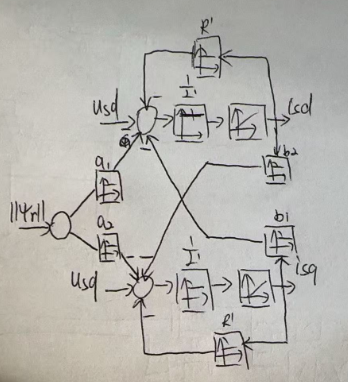
\includegraphics[width=0.5\textwidth]{figures/signal_flow_graph.png}
    \caption{Signal Flow Graph of the Stator Voltage Equations in d-q Frame}
    \label{fig:signal_flow_graph}
\end{figure}

 The values of $a_1\Psi_r^d+b_1I_s^q$ and $a_2\Psi_r^d+b_2I_s^d$ can be considered as disturbance inputs to the system. To eliminate the effects of these disturbances, we can use the feedforward control method. The compansated stator voltages are given in the next question.

\item 
The trnasfer functions $F_{i}(s)$ of the current and the desired voltages is:
\begin{equation}
    \begin{aligned}
    F_{i}(s)&=\frac{I_s^s}{U_s^{s*}(s)}=\frac{1}{R^{\prime}+L^{\prime}s}\cdot G_U(s)\\
        &=\frac{V_{i_s}V_{PE}}{(1+T_{i_s}s)\left(1+T_{PE}s\right)}
    \end{aligned}
\end{equation}
where $V_{i_s}=\frac{1}{R^{\prime}}=0.2014$, $T_{i_s}=\frac{L^{\prime}}{R^{\prime}}=5.522ms$, $V_{PE}=\frac{U_{DC}}{2}=280V$ and $T_{PE}=250\mu s$ are the gain and time constant of the power electronics.

and the desired voltages $U_s^{s*}(s)$ are:
\begin{equation}
    \begin{aligned}
        U_s^{d*\prime}(s)&=U_s^{d*}(s)-a_1\Psi_r^d(s)-b_1I_s^q(s)\\
        U_s^{q*\prime }(s)&=U_s^{q*}(s)-a_2\Psi_r^d(s)-b_2I_s^d(s)
    \end{aligned}
\end{equation}

Therefore, the parameters of the plant transfer function $F_{i}(s)$ are:
\begin{equation}
    \begin{aligned}
V_{i} & =V_{i_{s}}\cdot V_{PE}=\frac{1}{R^{\prime}}\cdot\frac{U_{DC}}{2}=56.38 \\
T_{1,i} & =T_{i_{s}}=\frac{L^{\prime}}{R^{\prime}}=0.0055\mathrm{s}=5.52\mathrm{ms} \\
T_{\sigma,i} & =T_{PE}=250\mathrm{\mu s}
\end{aligned}
\end{equation}

\item 
With information above, we can design the PI controller for the current control loop. It's a PT2 systm. Therefore, the parameters of the PI controller can be designed as:
\begin{equation}
    \begin{aligned}
        G_{PI,i}(s)&=V_{\mathrm{C,i}}\frac{1+sT_{\mathrm{n,i}}}{sT_{\mathrm{n,i}}}\\
        V_{C,i}&=\frac{T_{1,i}}{2T_{\sigma,i}\cdot V_i}=0.196\\
        T_{n,i}&=T_{1,i}=5.52\mathrm{ms}
    \end{aligned}
\end{equation}
\end{enumerate}
\subsection{ Flux and Rotor Speed Control}
\begin{enumerate}
\setcounter{enumi}{8}
\item 
The transfer function of the closed loop current control system is:
\begin{equation}
    F_{sub,i}(s)=\frac{I_s^s(s)}{I_s^{s*}(s)}=\frac{F_i(s)G_{PI,i}(s)}{1+F_i(s)G_{PI,i}(s)}=\frac{1}{1+s2T_{PE}s+s^2T^2_{PE}}
\end{equation}

where $T^2_{PE} \ll 1$ can be neglected. Therefore, the simplified transfer function of the closed loop current control system is:
\begin{equation}
    F_{sub,i}(s)=\frac{1}{1+sT_{equi,i}}
\end{equation}
where $T_{equi,i}=2T_{PE}=500\mu s$ is the equivalent time constant of the closed loop current control system.
\item 
From the differential equation of the rotor flux, we can derive the transfer function of the rotor flux as:
\begin{equation}
    F_{\Psi i}(s)=\frac{\Psi_r^d(s)}{i_s^{d}(s)}=\frac{L_m}{s+\frac{R_r}{L_r}}=\frac{V_{\Psi}}{1+sT_{\Psi}}
\end{equation}
where $V_{\Psi}=L_m=0.326$ and $T_{\Psi}=\frac{L_r}{R_r}=0.1172s$ are the gain and time constant of the rotor flux.

Considering the closed loop current control system, the transfer function from the desired d-axis current to the rotor flux is:
\begin{equation}
    F_{\Psi_r}(s)=\frac{\Psi_r^d(s)}{i_s^{d*}(s)}=\frac{V_{\Psi}}{(1+sT_{\Psi})(1+sT_{equi,i})}
\end{equation}

The small and large time constants are $T_{\sigma,\Psi_r}=T_{equi,i}=500\mu s$ and $T_{1,\Psi_r}=T_{\Psi}=0.1172s$ respectively.
\item 
It's a PT2 system. The parameters of the PI controller for the flux control loop can be designed as:
\begin{equation}
    \begin{aligned}
        G_{PI,\Psi}(s)&=V_{C,\Psi}\frac{1+sT_{n,\Psi}}{sT_{n,\Psi}}\\
        V_{C,\Psi}&=\frac{T_{1,\Psi}}{2T_{\sigma,\Psi}V_{\Psi}}=359.5\\
        T_{n,\Psi}&=T_{1,\Psi}=0.1172s
    \end{aligned}
\end{equation}
\setcounter{enumi}{13}
\item 
The transfer function of the speed loop can be derived as:
\begin{equation}
    \begin{aligned}
    F_{\omega}(s)=\frac{\omega(s)}{i_s^{q*}(s)} &=\frac{\hat{\omega}_m(s)}{{\omega}_m(s)}\cdot \frac{{\omega}_m(s)}{M_M(s)}\cdot \frac{M_M(s)}{i_s^{q}(s)}\cdot \frac{i_s^{q}(s)}{i_s^{q*}(s)}\\
        &=\frac{1}{1+sT_{f,\omega}}\cdot\frac{3}{2}p\frac{L_m}{L_{r}}\psi_{r,k} \cdot\frac{1}{\Theta_{m}s}\cdot \frac{1}{1+T_{equi,i}s}\\
        &=\frac{V_{S,\omega_{M}}}{T_{1,\omega_{M}}s(1+T_{\sigma,\omega_{M}}s)}
        \end{aligned} 
\end{equation}
    where $V_{S,\omega_{M}}=\frac{3\pi f_{N}L_m\psi_{rN}}{M_{MN}L_{r}}= 59.05$, $T_{1,\omega_{M}}=\frac{\Theta_M2\pi f_N}{pM_{MN}}=0.0951$ and $T_{\sigma,\omega_{M}}=T_{equi,i}+T_{f,\omega}=2.5ms$ are the gain, large and small time constants of the speed control loop.

\item
It's a IT1 system. The $M_{L}$ is disturbance input. we want SO optimization. Therefore, the parameters of the PI controller for the speed control loop can be designed as:
\begin{equation}
    \begin{aligned}
        G_{PI,\omega}(s)&=V_{C,\omega}\frac{1+sT_{n,\omega}}{sT_{n,\omega}}\\
        V_{C,\omega}&=\frac{T_{1,\omega}}{2T_{\sigma,\omega}V_{S,\omega}}=0.322\\
        T_{n,\omega}&=4T_{\sigma,\omega}=0.01s
    \end{aligned}
\end{equation}
\end{enumerate}
\end{document}
